\chapter{User Interfaces}

So far we have worked hard on the core mechanic of our game. Another important
aspect are the screens and components that wrap this mechanic. In this chapter
you will learn how to implement menus, popups and other user interface elements
in \cocos{}. 

\cocos{} provides its own set of basic UI components, such as buttons and
labels. For most games these components are sufficient. However, in this chapter
we also learn how to integrate Apple's UI framework \textit{UIKit}. Knowing
that is important for integrating many core Apple API's. As a specific example,
we will add integrate the Game Center framework in this chapter.

By the end of this chapter we will have a fully functional game!
Here's the basic screen flow our game will have:

\begin{figure}[H]
		\centering
		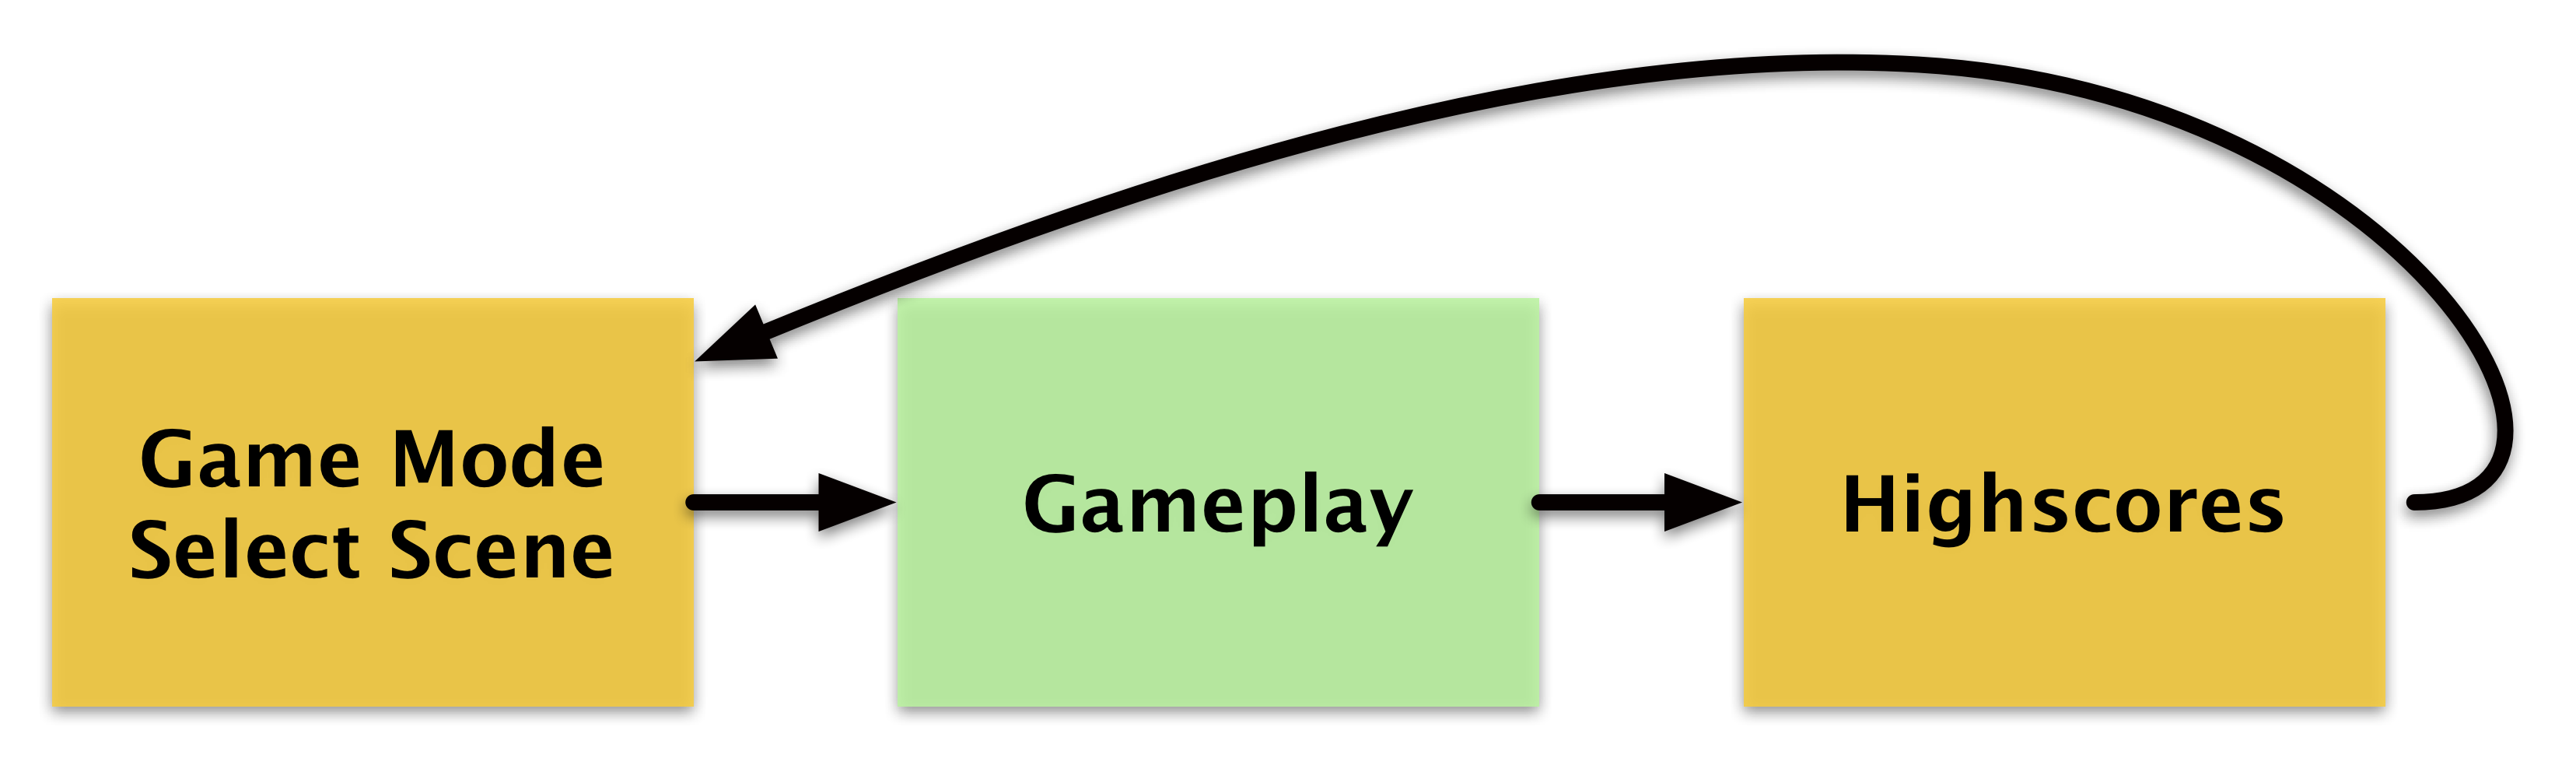
\includegraphics[width=0.7\linewidth]{images/Chapter6/screen_flow.png}
\end{figure}

Throughout this chapter you will not only learn how to build user interfaces
with \cocos{} and \SB{}, you will also learn how to structure this game to
support two different gameplay modes. We will implement and \textit{endless} and
a \textit{timed} gameplay mode, each with a different set of rules and
behaviors.

Let's start out by adding the game mode selection scene!

\section{Adding a game mode selection scene}
We will now change the screen flow of our existing game. Instead of diving into
the gameplay directly the user will see a game mode selection scene when
starting the game. 

The game mode selection scene will allow the user to swipe to switch between the
endless and timed game mode. Luckily \cocos{} provides a component called
\inlinecode{CCScrollView}\index{User Interface!CCScrollView} that implements
most of the functionality that we need for that scene.

\begin{leftbar}
Open the \SB{} project and create a new File (File -> New -> File\ldots). Name
the new file \textit{StartScene} and select \texit{Scene} as the type.
\end{leftbar}

We will create a game mode select scene that smoothly transitions into the
gameplay. To accomplish that we'll use the same background image for this scene
as for the actual gameplay. 

\begin{leftbar}
Drag the image \textit{backround.png} image onto the stage; it becomes the first
child of the root node of our new \textit{StartScene}.
\end{leftbar}

The background image should have exactly the same settings as in
\textit{MainScene} so that it fills the entire scene.

\begin{leftbar}
Select the background sprite in the timeline and apply the following steps:
\begin{enumerate}
  \item Set the position type for X to \textit{percentage of parent container}
  \item Set the X position to \textit{50}
  \item Set the position type for Y to \textit{percentage of parent container}
  \item Set the Y position to \textit{50}
\end{enumerate}
\end{leftbar}

Now the background image should fill the entire background. We will be
presenting some information in front of that background. To make that
information stand out more we will dim the background a little bit by turning
down its opacity. Since the fill color behind the background image is black a
lower opacity will result in a darker image.

\begin{leftbar}
Select the background sprite in the timeline. Set the opacity in the property
inspector to \textit{0.7}:
\begin{figure}[H]
		\centering
		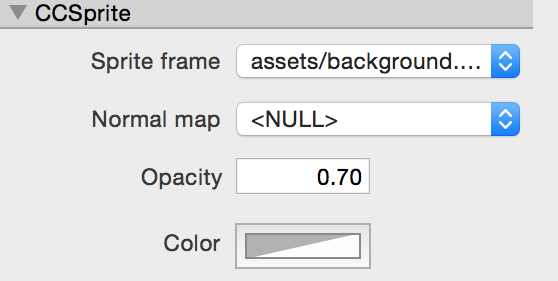
\includegraphics[width=200pt]{images/Chapter6/opacity_lower.png}
\end{figure}
\end{leftbar}

Next, we are going to add a label with an instruction for the player. A label is
a simple UI component that can display text. When building games with \cocos{}
we want to place the most UI components relative to screen edges. Using this
approach the UI will still look good when the game runs on a device with a
different screen size. Here's a little illustration:

\begin{figure}[H]
		\centering
		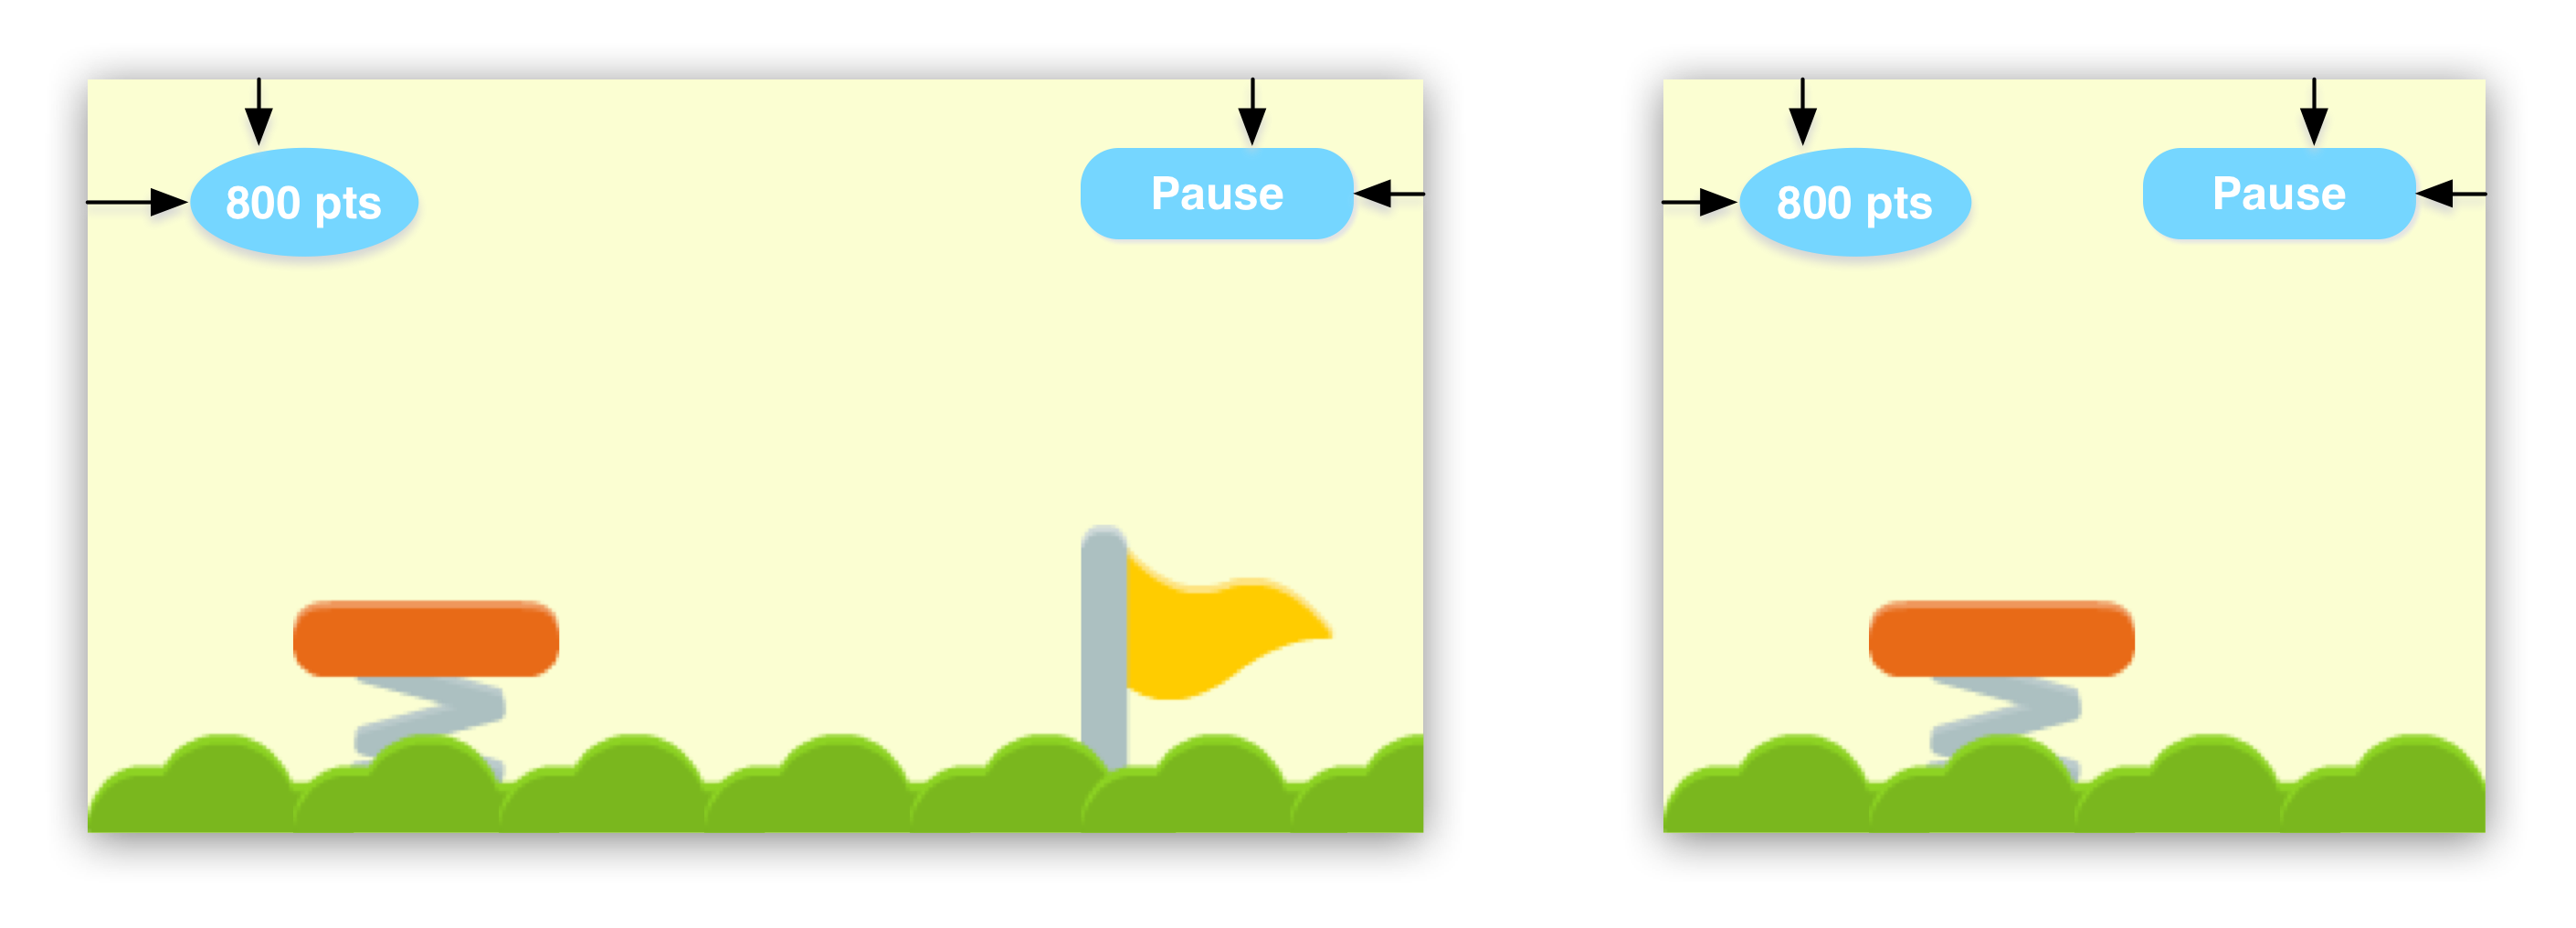
\includegraphics[width=0.7\linewidth]{images/Chapter6/multiple_screen_sizes.png}
		\caption{UI elements should be placed relative to screen edges to preserve
		their position on different screen sizes}
\end{figure}

Throughout this chapter we will use \cocos{}'s reference
corner feature to accomplish resizable user interfaces. 

\begin{leftbar}
Drag a \textit{CCLabelTTF} from the node library \textit{onto} the background
sprite, so that it becomes a child of it. Set the position up as following:
\begin{enumerate}
  \item Set the position to be relative from the \textit{Top-left}.
  \item Set the position type for X to \textit{percentage of parent container}
  \item Set the X position to \textit{50}
  \item Set the Y position to \textit{80}
\end{enumerate}

Set the label text to: \textit{Choose your game mode:}. We also want to change
the font and appearance of this label a little:
\begin{enumerate}
  \item As font name choose: \textit{Optima-Bold}
  \item As font size choose: \textit{40}
  \item Set the draw color to \textit{black}
  \item Set the outline color to \textit{white}
  \item Set the outline width to \textit{6}
\end{enumerate}
\end{leftbar}

After setting the label up your start scene should look as following:

\begin{figure}[H]
		\centering
		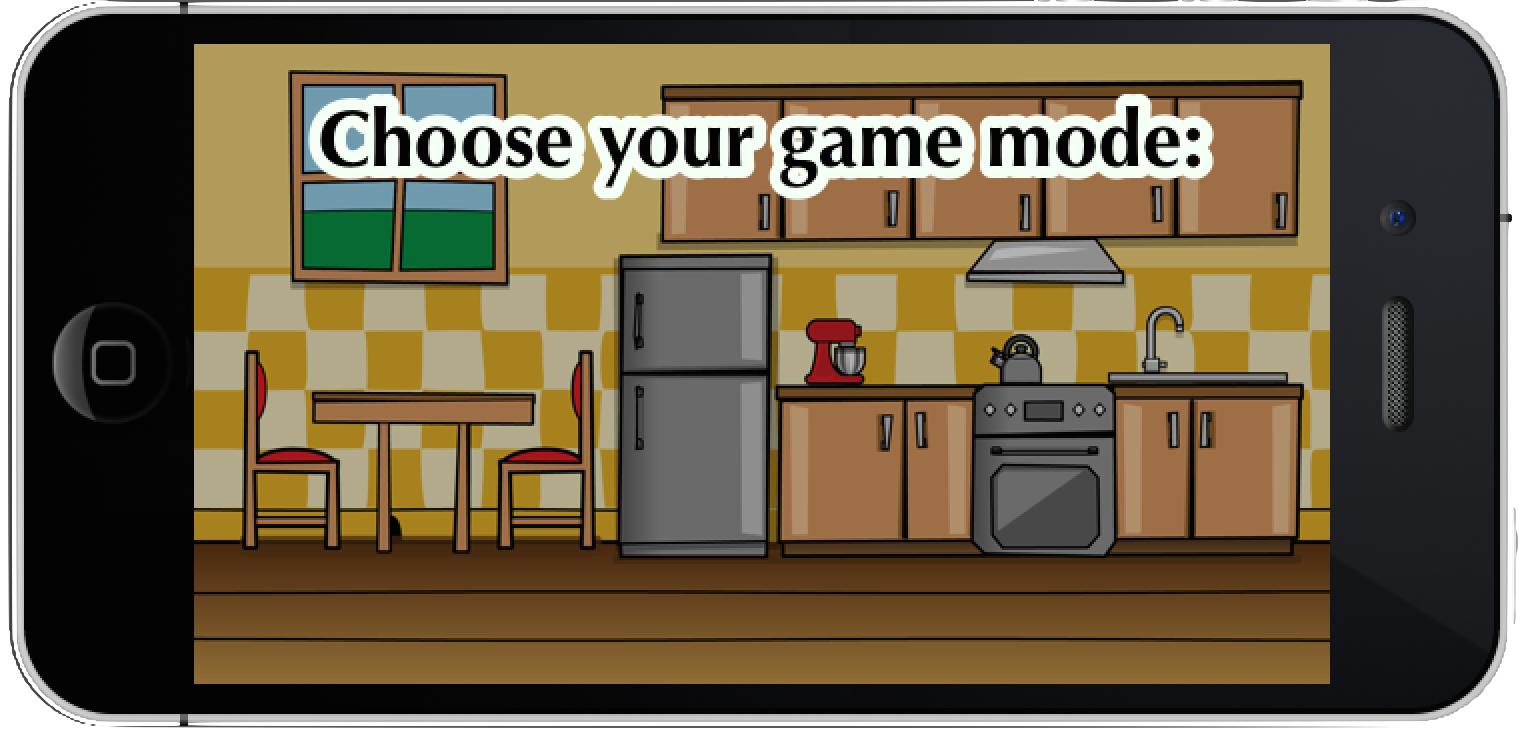
\includegraphics[width=0.7\linewidth]{images/Chapter7/start_scene.png}
		\caption{UI elements should be placed relative to screen edges to preserve
		their position on different screen sizes}
\end{figure}

There's a lot more work left to do! As mentioned earlier we will create a scroll
view that let's the user swipe between two different game modes. Every scroll
view has a content node. That content node is larger than the size of the scroll
view and the scroll view can be used to view different parts of this content
node. Here's an illustration:

\begin{figure}[H]
		\centering
		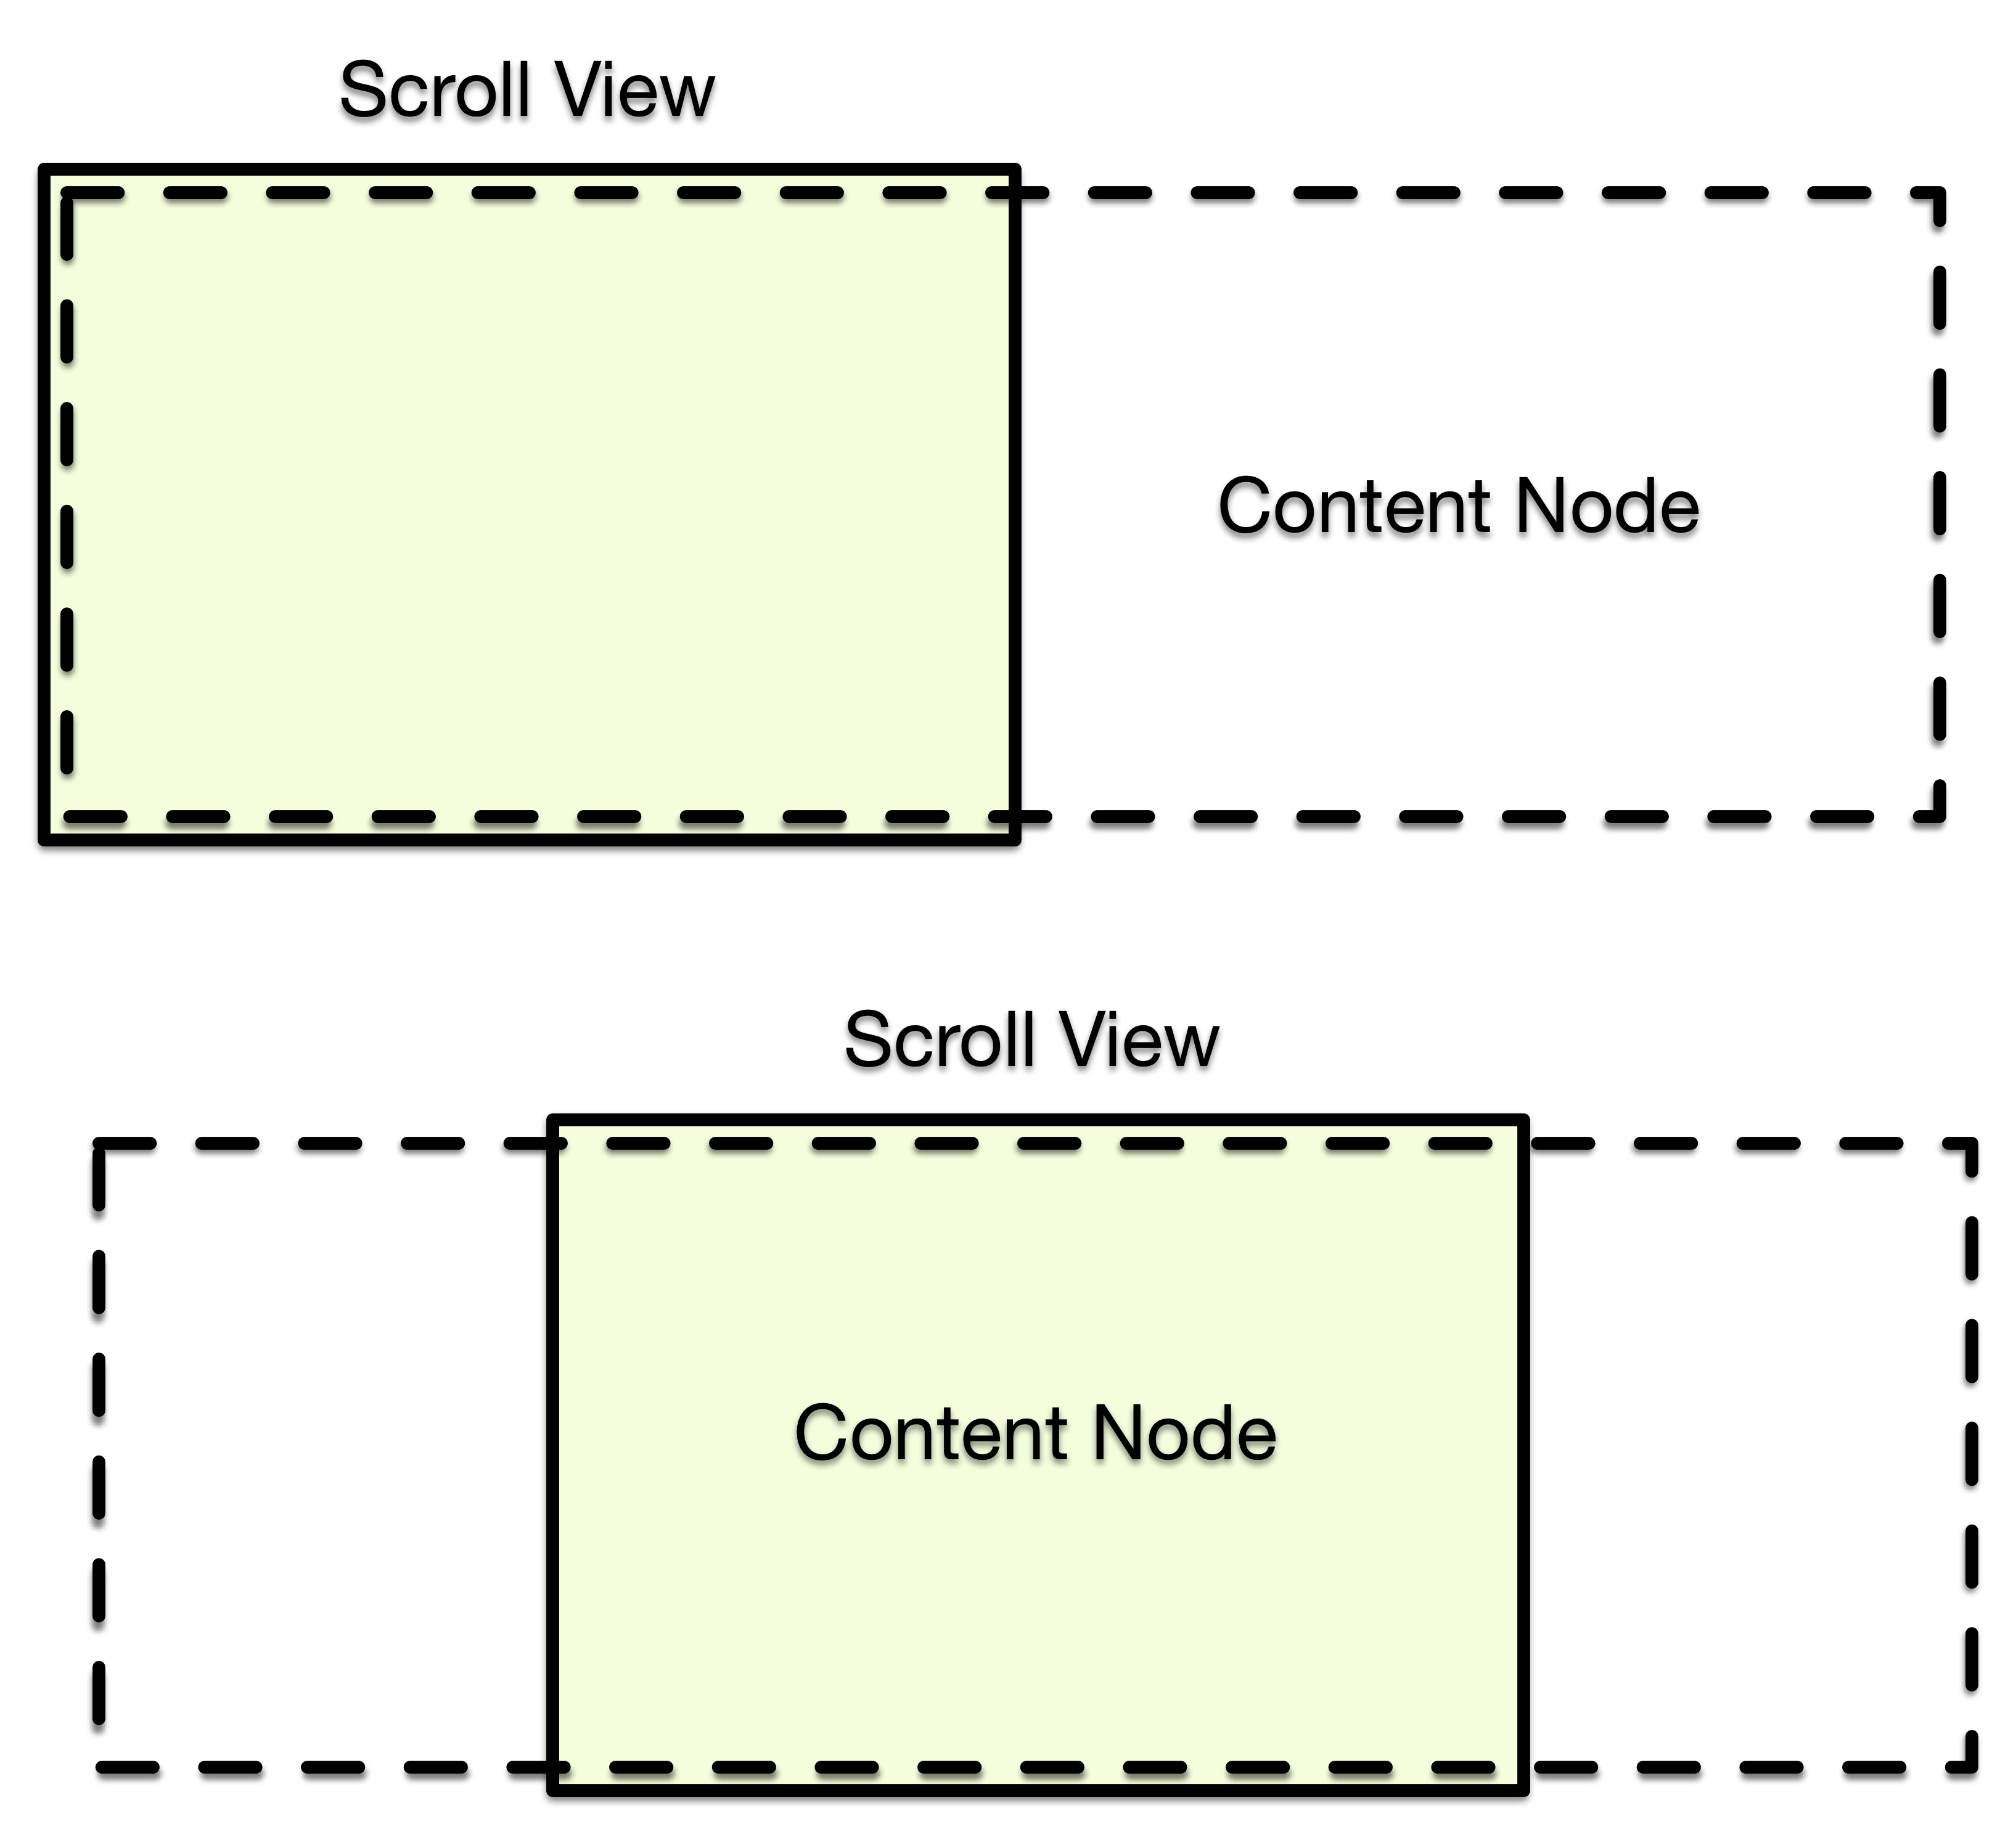
\includegraphics[width=0.5\linewidth]{images/Chapter7/scrollview_concept.png}
		\caption{The scroll view can present different portions of its larger content
		node. The user can change the displayed portion by swiping.}
\end{figure}

Our next step will be creating this content node. In general scroll views allow
users to scroll to any arbitrary position within the scroll view's content node.
In our specific example we would like to change this behavior. We only
want the user to select between two different game modes, each of these game modes will be
represented by a full screen node. It wouldn't make sense to allow the user to
scroll half way between the endless and timed game mode. For this specific case
the scroll view provides an option called \textit{Paging enabled}. If you want
to use a scroll view with paging your content node needs to have a size that is
a multiple of the scroll view's size. In our particular example the content node
for our scroll view will be twice as wide as the scroll view itself, resulting
in a scroll view with two pages. When paging is enabled, the scroll view will
always snap to one of the two pages as soon as a user stops scrolling. If this
sounds a little bit too abstract for you, it should become clearer as we implement and use the scroll view.

First we need to create the content view. We will set it up in a separate
\ccbfile{} file. 
\begin{leftbar}
Create a new \ccbfile{} called \textit{GameModeSelectLayer} and choose its type
to be a \textit{Layer}.
\end{leftbar}

\begin{details}[frametitle={Why are we using a Layer to create the scroll view
content?}]\index{Document Types}
A short refresher on the different \ccbfile{} types: Scenes are used to
represent full screen content. Sprites are used for simple Sprite Images. Nodes
are used for node compositions that don't have a specific content size. Layers
are used to create content within a stage that has a fixed size.
Layers are typically used for popups or scroll view content nodes because we
want to layout the content based on a container size. We can still use relative
positioning within layers. When the root node of the layer \ccbfile{} gets added
to another node its size will be determined and all relative layouts will be
applied accordingly. We'll use relative positioning for the content node we are
about to create.
\end{details}

\begin{leftbar}
Select the root node of \textit{GameModeSelectLayer.ccb} and choose the width
and height to be in percentage of the parent container. Choose 100\% for the
height and 200\% for the width of the node:
\begin{figure}[H]
		\centering
		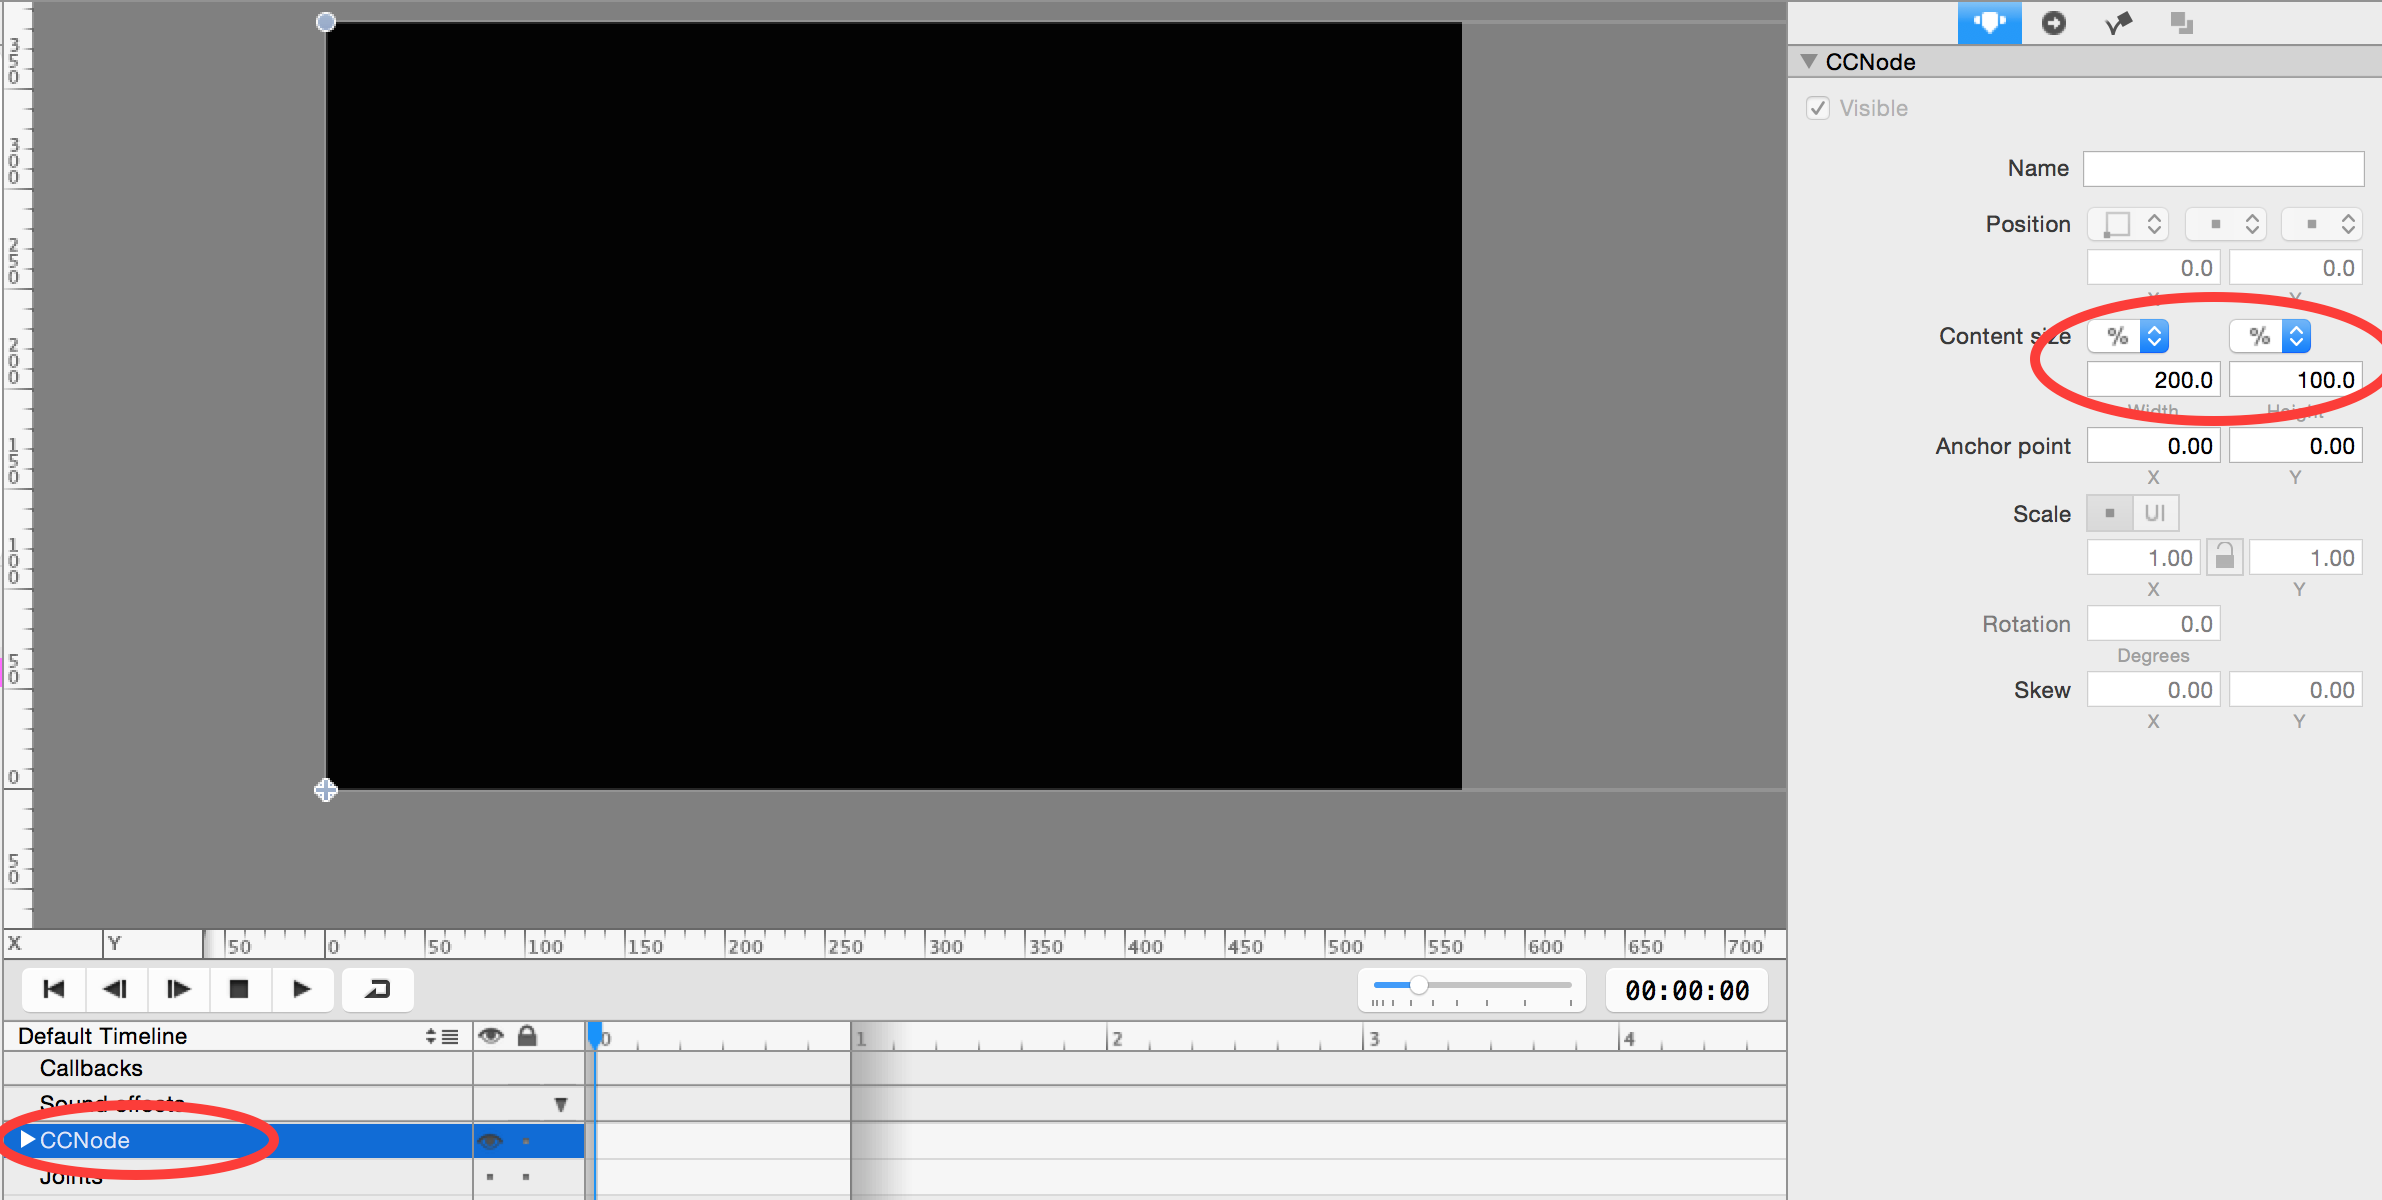
\includegraphics[width=0.6\linewidth]{images/Chapter7/content_node_width.png}
\end{figure}
\end{leftbar}
We want the scroll view to contain two pages, that means the content node needs
to be exactly double as wide as the scroll view. Because we are setting up the
size of the root node of this \ccbfile{} in percentage of the parent container,
its actual size will only be determined when it is added to a scroll view. This
is a great example of dynamic layouts; our scroll view could have any
arbitrary size and this content node would always be exactly twice as wide.

Inside of this root node we are going to place the content for our two different
pages. To provide a clean structure we will create one container node for each
page.

\begin{leftbar}
Add a \ccnode{} as a child to the root node. Name this child
\textit{endless-mode} by selecting the node in the timeline and hitting the
return key. Set the content type of the node to be in percentage of the parent
container. Set the width to 50\% and the height to 100\%. The container for the
left page is set up.
\end{leftbar}

\begin{leftbar}
Add a second \ccnode{} as a child to the root node. Name this child
\textit{timed-mode}. Set the content type of the node to be in percentage of the parent
container. Set the width to 50\% and the height to 100\%. Additionaly, set the x
position to be in percentage of the parent container and set the value to 50\%.
\end{leftbar}

Now we have containers for each page set up. We are going to fill them with
labels that describe the game mode represented on each page and an arrow
indicating that there is another game mode available by swiping across the
screen. This is what the completed content node will look like:

\begin{figure}[H]
		\centering
		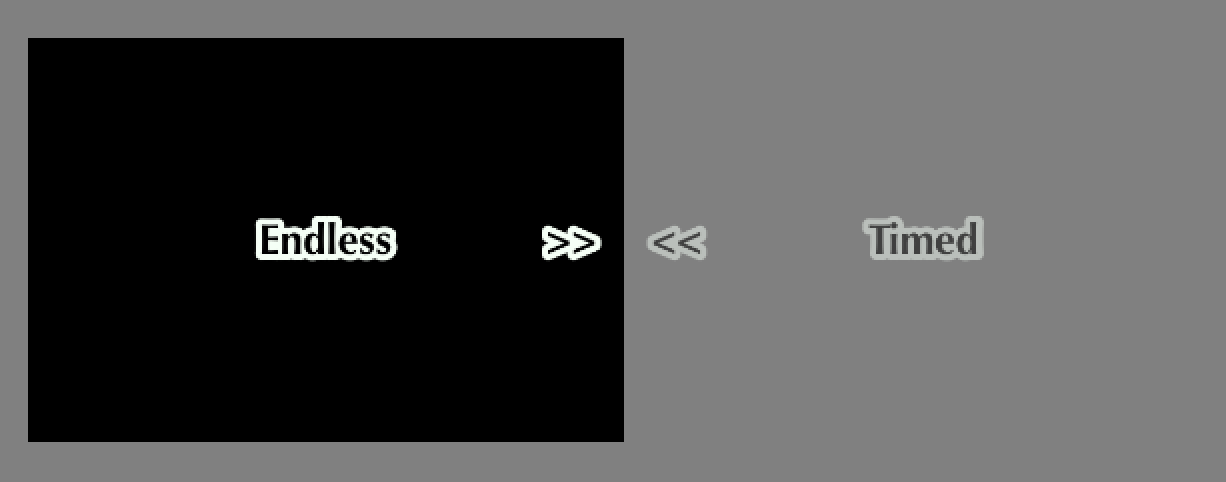
\includegraphics[width=0.6\linewidth]{images/Chapter7/content_node_completed.png}
		\caption{The completed content node by the end of this section.}
\end{figure}

First, let's add the labels for the endless mode.

\begin{leftbar}
Drag a \cclabel{} from the node library onto the \textit{endless-mode} node.
Center the label within its parent node by choosing a position type of
percentage of parent container. Then set x and y position to 50\%. This label
should look the same as the \textit{Choose your game mode} label on the start
scene. Apply the following settings:
\begin{enumerate}
  \item Set the label text to \textit{Endless}
  \item As font name choose: \textit{Optima-Bold}
  \item As font size choose: \textit{40}
  \item Set the draw color to \textit{black}
  \item Set the outline color to \textit{white}
  \item Set the outline width to \textit{6}
\end{enumerate}
\end{leftbar}

Next, let's add the arrow on the right side that will indicate that the player
can switch to the timed game mode.

\begin{leftbar}
Drag a \cclabel{} from the node library onto the \textit{endless-mode} node.
Apply the following settings:
\begin{enumerate}
  \item Set the label text to \textit{>>}
  \item As font name choose: \textit{Optima-Bold}
  \item As font size choose: \textit{40}
  \item Set the draw color to \textit{black}
  \item Set the outline color to \textit{white}
  \item Set the outline width to \textit{6}
  \item Set the position up as following: \begin{figure}[H]
										  \centering
										  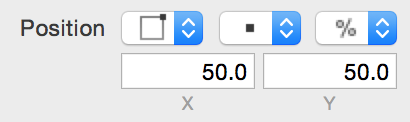
\includegraphics[width=150pt]{images/Chapter7/arrow_label_position.png}
										  \end{figure}
\end{enumerate}
\end{leftbar}

Now your stage should look like this:
\begin{figure}[H]
\centering
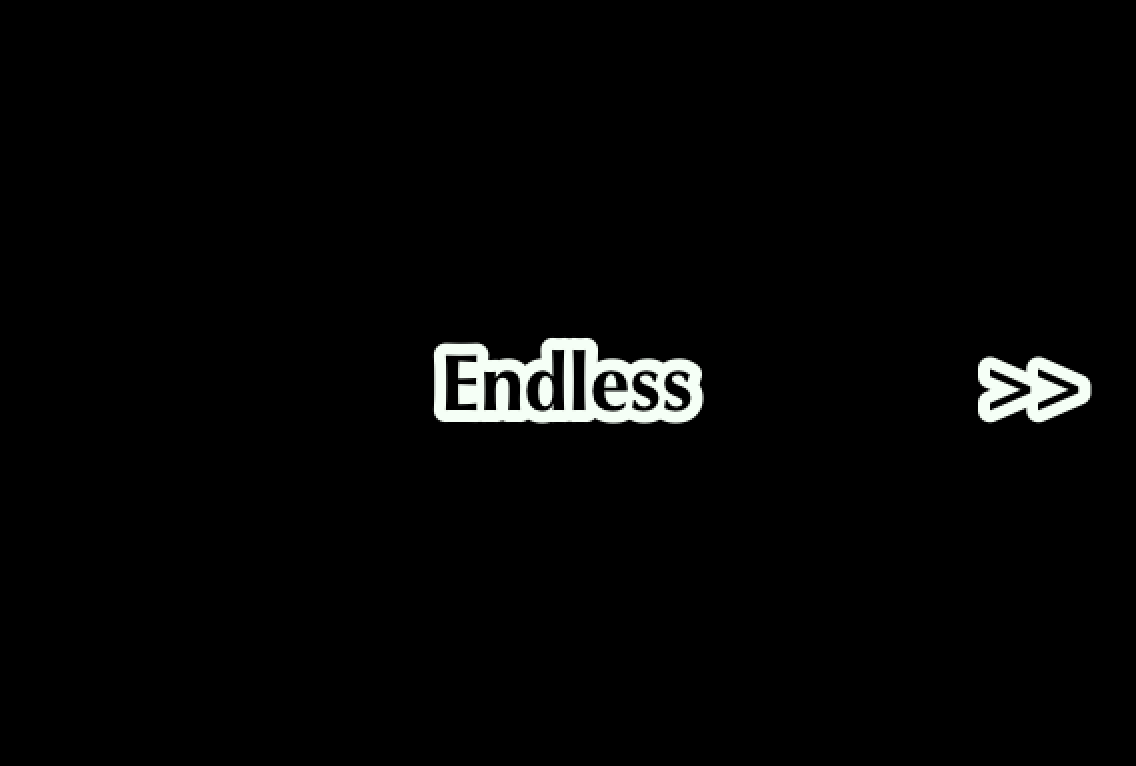
\includegraphics[width=150pt]{images/Chapter7/endless_mode.png}
\end{figure}
We're going to add a little visual detail to this game mode selection layer. The
arrows indicating the other available shall blink. This can be easily
accomplished using \SB{}'s timeline feature. 

\begin{leftbar}
Set the timeline duration to 1 second:
\begin{figure}[H]
\centering
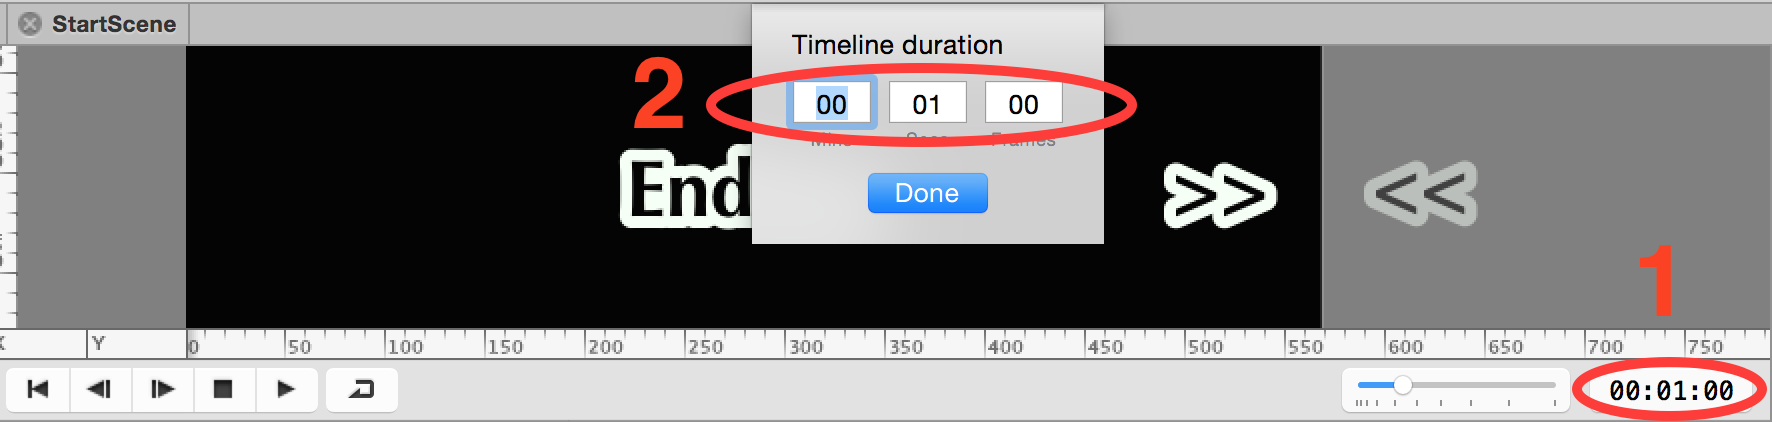
\includegraphics[width=300pt]{images/Chapter7/timeline_duration.png}
\end{figure}
\end{leftbar}

Now we are going to use three \textit{opacity} keyframes to create the blinking
animation. 
\begin{leftbar}
Select the label with the arrows in the timeline. Then create three
keyframes by hitting the \textit{O} (like in opacity) key on your keyboard.
Alternatively you can create keyframes through the top bar menu:
\textit{Animation -> Insert Keyframe\ldots -> Opacity}. Place the first keyframe
at 0 seconds the second one at 0.5 seconds and the third one at 1
second.
\end{leftbar}

Now we can set different opacity values for each of these keyframes and \SB{}
will create smooth animations between them. There are two ways to set a
specific value for a keyframe. You can select the keyframe and change the
relevant property in the property inspector in the right panel of \SB{}. The
easier way however is to double-click onto a keyframe. That will bring up a
small popup in which you can modify the relevant values:
\begin{figure}[H]
\centering
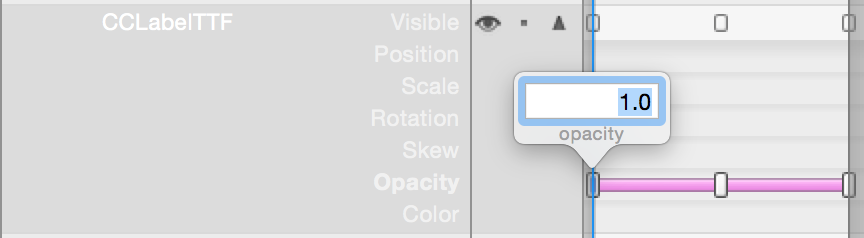
\includegraphics[width=250pt]{images/Chapter7/edit_keyframe.png}
\caption{Double-click onto keyframes to modify their values}
\end{figure}

\begin{leftbar}
Set the opacity in the first keyframe to 0. Set the opacity to 1 in the second
keyframe. For the third keyframe set the opacity to 1 again.
\end{leftbar}

Now the arrow will appear for half a second and then disappear for another half
a second. We don't want this animation to be over after 1 second. Instead we
want to loop it forever. We can do so by \textit{chaining}\index{\SB{}
Timeline!Chaining} the timeline to itself. In \SB{} timelines can be chained to
each other. That means that you can define that another timeline should run
after the current timeline is completed. If you use this feature to chain a
timeline to itself you have an endlessly running timeline animation!

\begin{leftbar}
Chain the default timeline to itself as shown below:
\begin{figure}[H]
\centering
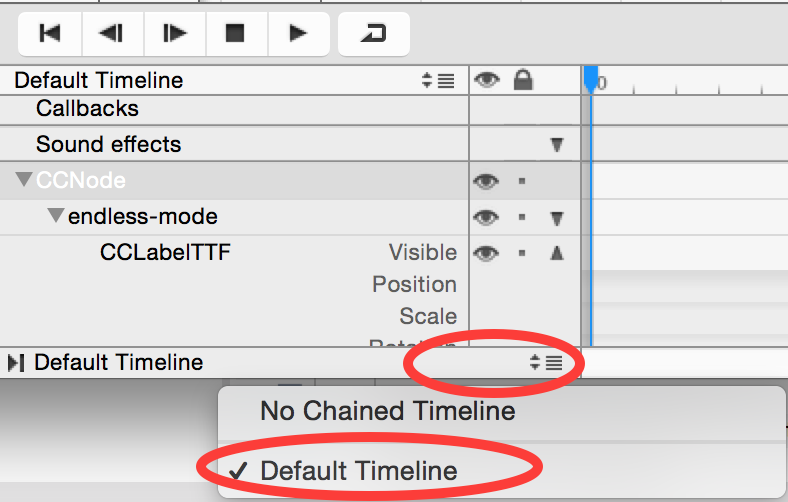
\includegraphics[width=200pt]{images/Chapter7/chain_timeline.png}
\caption{Double-click onto keyframes to modify their values}
\end{figure}
\end{leftbar}

\begin{details}[frametitle={Looping animations in \SB{}}]
Animations that are set up with a chained timeline will loop endlessly when your
game is running on a simulator or phone. In \SB{} itself the animation will only
run once. If you want to preview what your animation will look like when it is
looped, you need to use the following control in the timeline playback panel:
\begin{figure}[H]
\centering

\includegraphics[width=100pt]{images/Chapter7/loop_timeline.png}
\end{figure}
Note that this control will only affect your previewed animation in \SB{}. Not
the actual animation running in your game.
\end{details}

Now we are finished setting up one of the two game modes. Setting up the node
for the timed game mode involves exactly the same steps as you have seen just
now. The only difference is the arrow label. The arrows should be pointing to
the left and the arrow should be positioned from the left edge of the
\textit{timed-mode} node. I will leave this as an exercise to you. Remember that
you can always check the solution on GitHub if you get stuck. Once you have set
up the node for the second game mode come back and we'll integrate this game
mode selection layer into the start scene.

\begin{leftbar}
Switch to the \textit{StartScene.ccb} file and drag a \textit{CCScrollView} from
the node library onto the \textit{background} node. Set the position to 0,0. The
scroll view shall cover the entire screen, so set the size type to
\textit{percentage of parent container} and choose 100\% for the width and the
height of the scroll view. Set up the scroll view specific settings in the
property inspector as follows:
\begin{figure}[H]
\centering
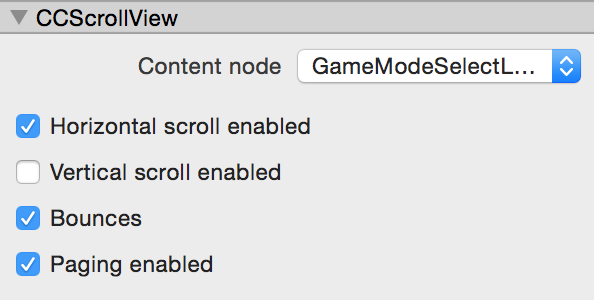
\includegraphics[width=250pt]{images/Chapter7/scrollview_settings.png}
\end{figure}
\end{leftbar}
Let's discuss the scroll view settings briefly. The most important property is
the \textit{Content node} property. Here you can choose a \ccbfile{} that will
be displayed inside of the scroll view. We choose the
\inlinecode{GameModeSelectLayer.cbb} that we just created. We check
\textit{Horizontal scroll enabled} because the user shall only be able to scroll
left and right, not up or down. We discussed the option \textit{paging enabled}
briefly at the beginning of this section. With this setting activated the scroll
view will always snap to one of the game modes and will not allow the user to
stop scrolling in the middle of two game modes.

Great! At this point the set up of our start scene is almost complete.
